\chapter{Rappresentazioni Numeriche e Testuali}

\section{Aritmetica Binaria}

I calcolatori utilizzano valori discreti (differenze di potenziale) fra 0 e 1 per rappresentare valori numerici. Viene detta Aritmetica Binaria l'aritmetica con i numeri rappresentati in base 2.

Siamo abituati a ragionare in base 10, ad esempio il numero 413 in base 10 è 
\[ 104 = 10^2 \cdot 1 + 10^1 \cdot 0 + 10^0 \cdot 4 \]

Lo stesso numero rappresentato in base 2 (codice binario) è

\[ 104_{10} = 01101000_2 = 2^7 \cdot 0 + 2^6 \cdot 1 + 2^5 \cdot 1 + 2^4 \cdot 0 + 2^3 \cdot 1 + 2^2 \cdot 0 + 2^1 \cdot 0 + 2^0 \cdot 0 \]

Un numero binario di 8 cifre è detto \textbf{byte}, un numero di 4 cifre è detto \textbf{nibble}. Una \textbf{parola} (\textbf{word}) è la quantità minima su cui viene rappresentato un intero in un calcolatore. Ad oggi le parole dei calcolatori sono 64 bit, alcuni calcolatori datati hanno parole da 32 bit.

La somma nell'aritmetica binaria è definita normalmente per i numeri positivi. Nei calcolatori i numeri hanno una dimensione finita (numero di bit) che indica il numero di cifre binarie con le quali è possibile rappresentare un numero. I positivi binari rappresentano numeri fino a $ 2^{N}-1 $ dove $ N $ è il numero di cifre.

Per rappresentare i numeri negativi si utilizza il metodo \textbf{segno-magnitudo} dove il bit più a sinistra rappresenta il segno (0 se il numero è positivo e 1 se è negativo). Il problema del metodo segno-magnitudo è che non rispetta la somma aritmetica. Può rappresentare numeri da $ [-2^{N-1}, +2^{N-1} ] $

Un metodo migliore per rappresentare i numeri negativi è il \textbf{complemento a due}. Nel complemento a due la cifra più a sinistra rappresenta sempre $ 2^{N-1} $ ma \textbf{negativo}. Il resto delle cifre sono positive e vengono sommate alla prima cifra negativa. Questo metodo rispetta la somma aritmetica. Per moltiplicare un numero per $ -1 $ si invertono le cifre binarie e si aggiunge 1 al numero. È possibile anche la sottrazione sommando un numero positivo ad uno negativo.

La somma fra due cifre può essere costruita con reti logiche. Il risultato della somma $ A + B = A \oplus B $ (operatore XOR) mentre il riporto della somma = $ A \land B $ (operatore AND)

\begin{figure}
	\centering
	\caption{Gate XOR}
	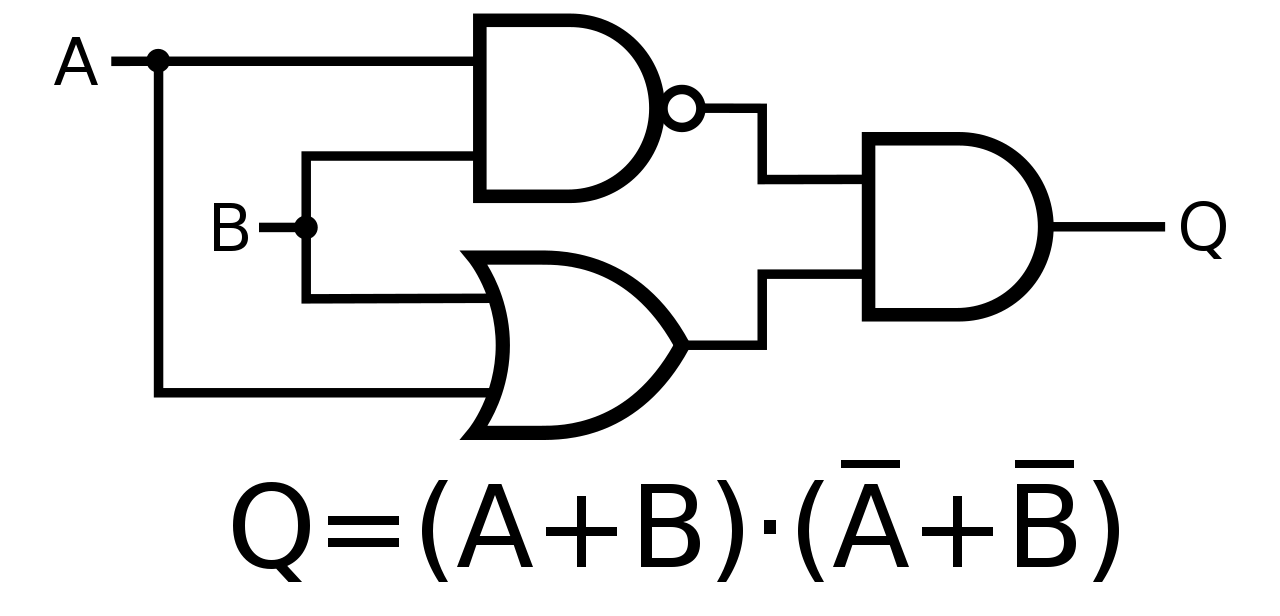
\includegraphics[width=\textwidth/2]{xor}
\end{figure}

\section{Esadecimale} 

I numeri esadecimali sono numeri in base 16. Siccome non bastano le cifre decimali per rappresentare i numeri maggiori di 9 si usano le prime lettere dell'alfabeto.
Una cifra esadecimale rappresenta un nibble (4 bit).

\section{Numeri in virgola mobile}

I numeri in virgola mobile si rappresentano con lo standard EEE 754 che definisce come si rappresentano i numeri in virgola mobile a singola precisione e doppia precisione (32 e 64 bit)

I bit del numero vengono divisi in 3 parti. Il primo bit denota il segno, la seconda parte rappresenta l'esponente e la terza parte si denota mantissa. L'esponente esprime dove la virgola verrà posizionata, come nella notazione scientifica di una calcolatrice l'esponente rappresenta $ 10^{n} $ dove $ n $ è l'esponente. La mantissa è un numero di base moltiplicato per $ 10^0 $, e viene successivamente moltiplicato per l'esponente.
L'esponente può essere sia positivo che negativo.

\begin{figure}
	\caption{Standard IEEE 754 a 32 bit}
	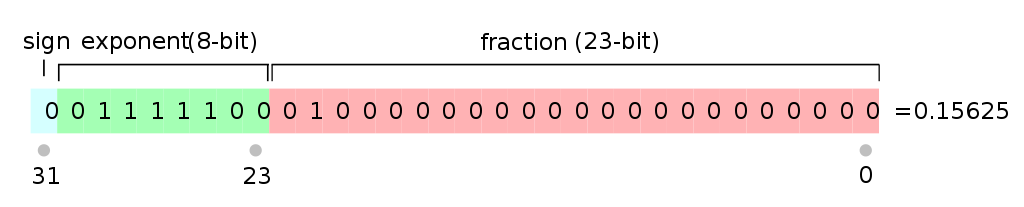
\includegraphics[width=\textwidth]{eee_floating_32}
\end{figure}

Nello standard a 32 bit la sezione esponente ha 8 bit di lunghezza. Un numero ad 8 bit può rappresentare numeri da 0 a 255, per ottenere gli esponenti negativi nello standard dei numeri a virgola mobile il numero a 8 bit rappresenta invece numeri da -127 a +128

\begin{figure}
	\caption{IEEE 754 a 64 bit}
	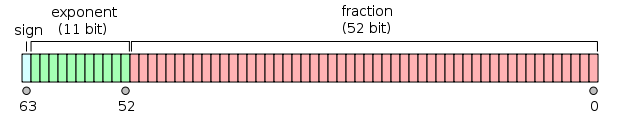
\includegraphics[width=\textwidth]{eee_floating_64}
\end{figure}

\paragraph{Somma dei numeri a virgola mobile}

Per sommare i numeri a virgola mobile il primo passo è allineare le mantisse, significa osservare gli esponenti e spostarli fino a che le cifre non sono sommabili in colonna.
Il secondo passo consiste nel sommare e il terzo passo nel normalizzare la somma. Nei processori la somma floating point viene eseguita in dei moduli appositi che in input ricevono due o più numeri floating point ed eseguono in dei sotto-moduli i tre passaggi della somma in un tempo $ 1/3 t $ dove $ t $ è il tempo totale per eseguire una somma. I tre passaggi della somma possono essere sequenzializzati così che una volta che ogni sotto-modulo ha completato il passo, può ricevere subito l'input successivo (la somma di due numeri FP impiegherà $ t + 1/3 $ invece che $ 2t $)

\paragraph{Estensioni vettoriali}
Alcuni processori permettono di eseguire operazioni contemporaneamente su un registro dividendolo in sottoregistri più piccoli. 

\section{Codifica ASCII}
La codifica ASCII è una tabella di codifica di caratteri testuali con interi da 0 a 255 (8 bit). La codifica ASCII estesa è a 16 bit e comprende diversi caratteri non latini.

\begin{figure}
	\caption{Tabella ASCII}
	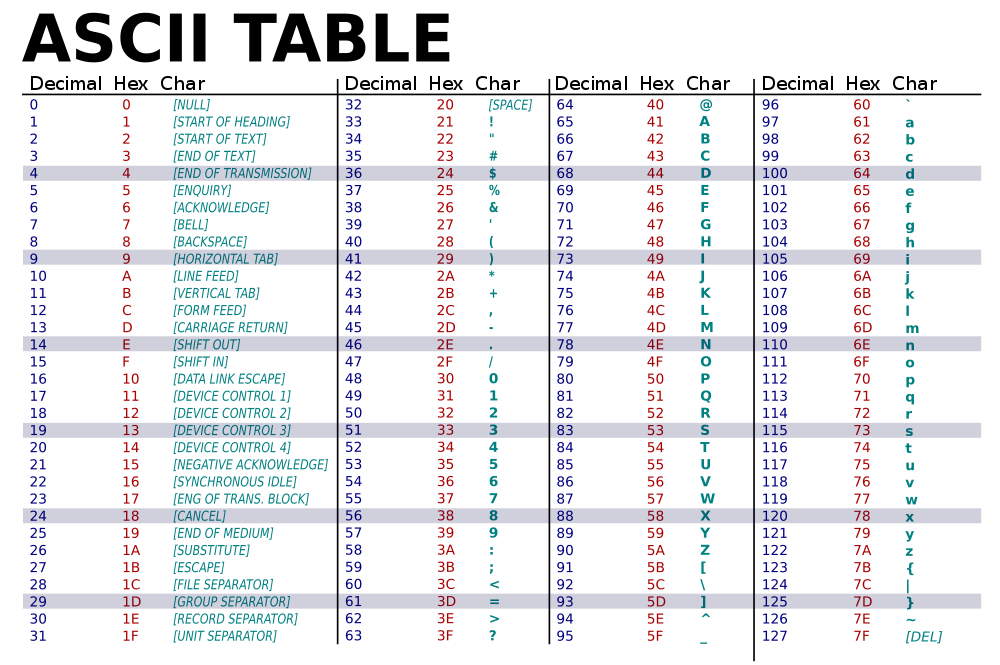
\includegraphics[width=\textwidth]{ascii}
\end{figure}